% [[file:../index.org::*System of Linear Equations][System of Linear Equations:1]]
%%%%%%%%%%%%%%%%%%%%%%%%%%%%%%%%%%%%%%%%%%%%%%%%%%%%% Lineare Gleichungssysteme %%%%%%%%%%%%%%%%%%%%%%%%%%%%%%%%%%%%%%%%%%%%%%%%%
\newpage

\section{System of Linear Equations}

%%%%%%%%%%%%%%%%%%%%%%%%%%%%%%%%%%%%%%%%%%%%%%%%%%%%%
% System of Linear Equations:1 ends here

% [[file:../index.org::*Some Examples to Start With][Some Examples to Start With:1]]
\subsection{Some Examples to Start With}

\label{Einleitungsbeispiele}
Look at the following four problems. You don't have to solve these problems yet, just formalize them, i.e. find the 
equations which describe the situation. 


\begin{exer}\label{exer1}
Two types of coffee: the first one costs 18 Swiss francs per kilo, the second 25 Swiss francs per kilo. We have to produce a mixture of 5 kilos. How much coffee of each type must be selected for the mixture to cost 20 Swiss francs per kilo?
\end{exer}
\vspace{5\baselineskip}

\begin{exer}\label{exer2}
Five years ago the father was 5 times as old as the son was then, and in 3 years the father will be 3 times as old as the son. How old are they now?
\end{exer}
\vspace{5\baselineskip}

\begin{exer}\label{exer3}
Two farmers have sheep. If the first gives a sheep to the second, both have the same number. But if the second gives a sheep to the first, the first has twice as many as the second. How many sheep does everyone have?
\end{exer}
\vspace{5\baselineskip}

\begin{exer}\label{exer4}
A three-digit natural number has a checksum (Quersumme) of 18. If the first digit (from the left) is swapped with the second digit, the number grows by 180, but if the second digit is swapped with the third digit, the number grows by 18. What is the number called?
\end{exer}
\vspace{5\baselineskip}
\newpage
%%%%%%%%%%%%%%%%%%%%%%%%%%%%%%%%%%%%%%%%%%%%%%%%%%%%%
% Some Examples to Start With:1 ends here

% [[file:../index.org::*System of Linear Equations][System of Linear Equations:1]]
\subsection{System of Linear Equations}

In the above examples, one equation was not enough to describe the situation. We needed two or even three. This is called a \textbf{system} of equations. 
\vsp


\begin{tcolorbox}[colback=white]
\begin{definition}
A \textbf{$m\times n$-system of equations} is a set of $m$ equations which all contain the same $n$ variables. The system is called \textbf{linear (SLE)} if all equations are linear. 
\end{definition}
\end{tcolorbox}
\vsp

Before we start to solve such a system of linear equations, we standardize the way that we write down these systems to make them easier to be solved:
\vsp

\begin{tcolorbox}[colback=white]
We denote the SLE in the so-called \textbf{normal form}: 
\begin{itemize}
\item On the left-hand side of the equation sign are all terms with variables, denoted in an alphabetical order. 
\item On the right-hand side of the equation sign are all terms with only numbers. 
\end{itemize}
\end{tcolorbox}
\vsp

\begin{example}
\[
\begin{array}{ll}
\text{any form}\\
\\
2x+3y-8=0 \\
x+3=2y 
\end{array}
\hsp\Rightarrow\hsp
\begin{array}{ll}
\text{normal form}\\
\\
2x+3y=8 \\
x-2y=-3 
\end{array}
\]
\end{example}
\vsp

\begin{exer} 
Denote the systems of linear equations of exercises \ref{exer1}-\ref{exer4} in the normal form.
\end{exer}

\newpage
%%%%%%%%%%%%%%%%%%%%%%%%%%%%%%%%%%%%%%%%%%%%%%%%%%%%%
% System of Linear Equations:1 ends here

% [[file:../index.org::*The Solution of a System of Linear Equations][The Solution of a System of Linear Equations:1]]
\subsection{The Solution of a System of Linear Equations}
What does it mean to solve a system of linear equations? 
\vsp

\begin{tcolorbox}[colback=white]\begin{definition}
A solution of a system of linear equations with $n$ variables is given by an ordered tuple of $n$ values: If we insert these $n$ values into the variables, all equations will be correct simultaneously (i.e. all of them denote a correct statement).
\end{definition}
\end{tcolorbox}
\vsp

\begin{example}
Let's have a look at the following system of linear equations:
\begin{itemize}
\item[(I)] $x+2y=7$
\item[(II)] $2x-y=-1$
\end{itemize}
If we insert $1$ for $x$ and $3$ for $y$, the two equations denote a correct statement:
\begin{itemize}
\item[(I)] $1+2\cdot 3=7$
\item[(II)] $2\cdot 1-3=-1$
\end{itemize}
Therefore, $(1/3)$ is a solution of the system of linear equations.Actually, it is the only correct solution (which we cannot yet prove)which means that
\[
\mathbb{L}=\{(1/3)\}.
\]
\end{example}
\vsp

\begin{example}
Let's consider the following system of linear equations:
\begin{itemize}
\item[(I)] $x+y+2z=4$
\item[(II)] $-x+3y+4z=1$
\item[(III)] $2x+y=3$.
\end{itemize}
If we insert $2$ for $x$, $-1$ for $y$ and $1.5$ for $z$, we get correct statements for all three equations:
\begin{itemize}
\item[(I)] $2+(-1)+2\cdot 1.5=4$
\item[(II)] $-2+3\cdot (-1)+4\cdot 1.5=1$
\item[(III)] $2\cdot 2+(-1)=3$
\end{itemize}
Therefore, $(2/-1/1.5)$ is a solution of this system of linear equations. Again, it is the only solution (which we still can't prove yet) and therefore
\[
\mathbb{L}=\{(2/-1/1.5)\}.
\]
\end{example}


\newpage
\begin{exer}$ $

\begin{enumerate}[label=\emph{\alph*})]
\item	A $4\times 4$-SLE may be solved by inserting the four values 1, -3, 4 and 17 for the variables. Write down the correct notation for the solution.
\vfill

\item	Invent an exercise with the only solution $(1 / -5)$.
\vfill

\item	Invent an exercise with solution set $\{1,-5\}$.
\vfill

\item	A few students solved a $3\times 3$-SLE. Some of the answers are clearly wrong. Which ones?

\begin{tabular}{ll}
Anna: & $\mathbb{L}=\{-4,6,12.5\}$\\ 
Beat: &$x=-4$\\ 
Claude:  &$\mathbb{L}=\{(-4/6/12.5)\}$\\
David:  &Solution:$(-4/6)$\\ 
Ernest:  &$x=-4, y=6, z=12.5$
\end{tabular}
\vfill
\end{enumerate}
\end{exer}



\newpage
%%%%%%%%%%%%%%%%%%%%%%%%%%%%%%%%%%%%%%%%%%%%%%%%%%%%%
% The Solution of a System of Linear Equations:1 ends here

% [[file:../index.org::*How to Solve a SLE][How to Solve a SLE:1]]
\subsection{How to Solve a SLE}

To solve a SLE we need to find values for all variables such that all equations are solved simultaneously. But how can we find such a solution of the system of linear equations without guessing or simple trial and error?? There are two methods we will look at: the substitution method and the elimination method. But before we look at these methods, you should think about the problem yourself: How could you solve the following two systems of linear equations:


\begin{exer}\label{exer:SLE}
$ $

\vsp

\begin{enumerate}[label=\emph{\alph*})]

\item 
\begin{itemize}
\item[(I)] $3x-y =-1$
\item[(II)] $-6x+7y=12$
\end{itemize}
\vfill

\item 
\begin{itemize}
\item[(I)] $x+y+z=2$
\item[(II)] $2x-y+z=-1$
\item[(III)] $-x+2y-3z=6$
\end{itemize}

\end{enumerate}
\vfill
\end{exer}




%%%%%%%%%%%%%%%%%%%%%%%%%%%%%%%%%%%%%%%%%%%%%%%%%%%%% 
\newpage
% How to Solve a SLE:1 ends here

% [[file:../index.org::*The Substitution Method][The Substitution Method:1]]
\subsubsection{The Substitution Method}

The name of this method gives us a hint of what's going on: ``substituere'' means ``replacing'', ``inserting''.  
\vsp

\begin{example}
To solve the $2\times 2$-system of the above exercise \ref{exer:SLE}, we solve the first equation for $y$
\[
(I) \hsp 3x-y=-1 \hsp \Leftrightarrow \hsp 3x=y-1 \hsp\Leftrightarrow \hsp y=3x+1
\]
and use this result by replacing the $y$ in the second equation by the result we just got:
\[
(II) \hsp  -6x+7\cdot (3x+1) =12
\]
We got a linear equation in one variable which is easy to solve:
\[
(II) \hsp\Leftrightarrow\hsp -6x+21x+7=12 \hsp\Leftrightarrow\hsp 15x=5 \hsp\Leftrightarrow\hsp x=\frac13
\]
Again, we use the result for $y$ we got from the first equation (I) which gives 
\[
y=3x+1=3\cdot \frac 13+1 = 2
\]
Therefore, the solution is given by $x=\frac{1}{3}$ and $y=2$, i.e. by the 2-tuple $(\frac13/ 2)$.
\end{example}
\vsp\vsp

\begin{example}
To solve the $3\times 3$-system of the above exercise \ref{exer:SLE}, we solve one of the equations for one variable, for example $z$, and use this result by entering it into the two other equations to get a $2\times 2$-system:
\[
(I)\hsp x+y+z=2 \hsp\Leftrightarrow\hsp z=2-x-y
\]
Replace $z$ in the two other equations:
\[
\begin{array}{lrcl}
(II) &2x-y+(2-x-y)&=&-1\\
(III)  &-x+2y-3\cdot(2-x-y)&=&6
\end{array}
\]
Simplifying the equations a bit, we get
\[
\begin{array}{lrcl}
(II)&x-2y &=&-3 \\
(III)&2x+5y&=&12
\end{array}
\]
We get a $2\times 2$-system. Apply the same procedure again to this new system: Solve equation (II) for $x$: 
\[
x=2y-3 \hspace{3cm} (*)
\]
Replacing $x$ by this solution in equation (III) gives
\[
2(2y-3)+5y=12 \hsp\Rightarrow\hsp 4y-6+5y=12 \hsp\Rightarrow\hsp 9y=18 \hsp\Rightarrow\hsp y=2.
\]
Insert this result into equation (*) to get the solution for $x$:
\[
x=2\cdot 2-3=1
\]
Now insert these results into equation (I) to get
\[
z=2-1-2=-1.
\]
The solution of the system of linear equations is therefore $(1/2/-1)$. Notice that the order of the numbers is important. The value of $x$ always comes first, then the value of $y$ and then the one of $z$. 
\end{example}

\vsp\vsp

Now it should be clear how to solve an arbitrary $n\times n$-system:


\begin{tcolorbox}[colback=white]

\textbf{The Substitution Method}:

\begin{itemize}
\item	Solve one of the equations (for examples the first one) with respect to one variable:
\[(I) \hsp \Leftrightarrow \hsp x=\framebox[1.1\width][l]{\text{term without x}}\]
\item	Replace (substitute) in all other equations the $x$'s by that term you got. Simplify these equations.
\item We get a $(n-1)\times(n-1)$-system. Repeat the steps above till you get a linear equation in just one variable and solve this equation.
\item Enter the solution in reverse order into the solutions you got for the variables to get all values of the variables and therefore a solution of the system. 
\end{itemize}
\end{tcolorbox}

\vsp

\begin{remark}
You need to be a bit careful when applying the substitution method:

Assume that $3(x-1)+y=x+5$ is an equation of a SLE. Solving this equation for $y$, we get $y=8-2x$. Now we should replace $y$ in all the other equations by that term. But what happens if we enter this term by accident into this equation itself?

\[
3(x-1)+(8-2x)=x+5 \hsp\Leftrightarrow\hsp 3x-3+8-2x=x+5 \hsp\Leftrightarrow\hsp x+5=x+5
\]

Of course, we get a correct statement, but not one which is very helpful. This equation is true for every value of $x$. The information of the equation is kind of lost. Therefore: Never use the same equation again after solving one equation for a variable. This equation has been exhausted and should not be used again. 
\end{remark}
\vsp\vsp

\begin{exer}
Solve the four examples \ref{exer1}-\ref{exer4} on page \pageref{Einleitungsbeispiele} with the substitution method.
\end{exer}

\newpage

%%%%%%%%%%%%%%%%%%%%%%%%%%%%%%%%%%%%%%%%%%%%%%%%%%%%%
% The Substitution Method:1 ends here

% [[file:../index.org::*The Elimination Method][The Elimination Method:1]]
\subsubsection{The Elimination Method}
The main goal when solving a system of linear equations is to get rid of variables. This can be done by substitution. But often there are easier ways to do so. The elimination method adds equations together to get new equations with fewer variables. 

\begin{example}
Let's have a look at the following $2\times 2$-system:
\[
\begin{array}{lrcl}
(I) &3x-y &=&-1\\
(II) &-6x+7y&=&12\\
\end{array}
\]

We transform the first equation a little bit by multiplying both sides of the equation by 2:
\[
\begin{array}{lrcl}
(I)'&6x- 2y &=&-2\\
(II)&-6x+7y&=&12\\
\end{array}
\]
 
If we add the two equations together (i.e. the left and the right-hand sides of the equations) we get a new equations which is correct as long as (I) and (II) are correct. But this new equation is much easier than the original ones, since it contains only one variable:

\[
2\cdot (I)+(II) \hsp\Leftrightarrow\hsp (I)'+(II) \hsp\Leftrightarrow\hsp 5y=10
\]

Therefore, $y=2$.

Entering this solution for $y$ into either (I) or (II) we get $x=\frac{1}{3}, y=2$.
\end{example}
\vsp


\begin{example} 
Let us consider a $3\times 3$-system. We have to do the procedure twice to get two equations in two variables:
\[
\begin{array}{lrcl}
(I)&x+y+z&=&2\\
(II)&2x-y+z&=&-1\\
(III)&-x+2y-3z&=&6
\end{array}
\]
 
Adding (I) and (III) gives an equation without $x$. 
\[
(I)+(III) \hsp\Leftrightarrow\hsp 3y-2z=8
\]

By multiplying (I) by $-2$ and adding this new equation and (II) together, we get:
\[
(-2)\cdot (I)+(II) \hsp\Leftrightarrow\hsp -3y-z=-5
\]

Now, the system has ``one dimension less''. We got two new equations in just two variables:
\[
\begin{array}{lrcl}
(I)'&3y-2z&=&8\\
(II)'&-3y-z&=&-5\\
\end{array}
\]	 

Adding these two equations together, we get
\[
(I)'+(II)' \hsp\Leftrightarrow\hsp -3z=3
\]
and therefore $z=-1$. Now we use this solution to get the solutions for $x$ and $y$:
\[
\begin{array}{l}
(I)' \hsp\Leftrightarrow\hsp 3y-2\cdot (-1)=8 \hsp\Leftrightarrow\hsp y=2\\
(I)  \hsp\Leftrightarrow\hsp x+2+(-1)=2 \hsp\Leftrightarrow\hsp x=1\\
\end{array}
\]
Of course, we could have used $(II)'$ and $(II)$ or $(III)$ as well instead of $(I)'$ and $(I)$. The solution of the SLE is $(1/2/-1)$.
\end{example}


\begin{tcolorbox}[colback=white]
\textbf{The Elimination Method}:

An arbitrary $n\times n$-system may be solved by
\begin{itemize}
\item multiplying (I) and (II) by appropriate numbers and adding them to eliminate a variable, for example $x$,
\item multiplying (I) and (III) by appropriate numbers and adding them to eliminate the same variable,
\item multiplying (I) and (IV) by appropriate numbers and adding them to eliminate the same variable,
\item $\ldots$
\item multiplying (I) and (n) by appropriate numbers and adding them to eliminate the same variable,
\end{itemize}

We get a $(n-1)\times(n-1)$-system which does not include one variable (in our case $x$) anymore. 

Repeat the whole procedure till you get a $1\times 1$-system. 

Insert the solution you get for the last variable into one of the equations of the $2\times 2$-system to get the solution of the second last variable. Insert these two solutions in one of the equations of the $3\times 3$-system to get the solution of the third last variable and so on till you get the solutions of all variables.
\end{tcolorbox}
\vsp

\begin{remark}
Of course, there are always several ways in which to solve such a system. You can also mix the substitution and elimination method. Often there are shortcuats and if you see them, you can solve the system much quicker than by just applying the same method all the time. 

Mathematicians always try to find neat ways how to solve riddles, so feel free to be creative: Have a close look at the system before solving it and try to find the shortest way how to solve it. By the way, solving it like that makes much more fun!
\end{remark}


\vsp
\begin{exer}
Solve the four examples \ref{exer1}-\ref{exer4} on page \pageref{Einleitungsbeispiele} with the elimination method.
\end{exer}

\newpage
%%%%%%%%%%%%%%%%%%%%%%%%%%%%%%%%%%%%%%%%%%%%%%%%%%%%%
% The Elimination Method:1 ends here

% [[file:../index.org::*Exercises][Exercises:1]]
\subsubsection{Exercises}
%\setlength{\baselineskip}{1.4\baselineskip}
\label{Uebungen}

\begin{exer}
Solve the following linear 2x2-systems using the substitution or the elimination method.

\begin{enumerate}[label=\emph{\alph*})]
\item 
\begin{itemize}
\item[(I)] $3x-y=-6$
\item[(II)] $2x+3y=7$
\end{itemize}
\vfill

\item
\begin{itemize}
\item[(I)] $2x-5y=10$
\item[(II)] $4x+3y=7$
\end{itemize}
\vfill

\item
\begin{itemize}
\item[(I)] $\frac 23 x + \frac15 y = 6$
\item[(II)] $\frac 16 x-\frac 12 y = -4$
\end{itemize}
\vfill

\item
\begin{itemize}
\item[(I)] $\frac 14 x - \frac 56 y = 5$
\item[(II)] $\frac45 x-y=11$
\end{itemize}
\end{enumerate}
\end{exer}
\vfill

\begin{comment}
\newpage
\begin{exer}
Write down the following systems in the normal form and solve them afterward:
\begin{enumerate}[label=\emph{\alph*})]
\item  
\begin{itemize}
\item[(I)] $\frac{2x-1}{3}+\frac{y+2}{4}=4$
\item[(II)] $\frac{x+3}{2}-\frac{x-y}{3}=3$
\end{itemize}
\vfill

\item
\begin{itemize}
\item[(I)] $(x+5)(y-2)=(x+2)(y-1)$
\item[(II)] $(x-4)(y+7)=(x-3)(y+4)$
\end{itemize}
\vfill


\item
\begin{itemize}
\item[(I)] $\frac{x+11y}{5}-9\cdot \frac{y+2}{4}=\frac 12$
\item[(II)] $\frac{x}{20}+\frac 56= \frac{x}{15}+\frac{y}{10}$
\end{itemize}
\vfill

\end{enumerate}
\end{exer}
\end{comment}

\newpage
\begin{exer}
Solve the following systems with respect to $x$ and $y$. $t, r$ and $s$ are a parameters.

\begin{enumerate}[label=\emph{\alph*})]

\item
\begin{itemize}
\item[(I)] $2x-3y=9t$
\item[(II)] $4x-y=8t$
\end{itemize}
\vfill

\item
\begin{itemize}
\item[(I)] $2x-y=-5s$
\item[(II)] $3x+2y=7r-4s$
\end{itemize}
\vfill

\end{enumerate}
\end{exer}

\newpage
\begin{exer}
$ $

\begin{enumerate}[label=\emph{\alph*})]

\item
\begin{itemize}
\item[(I)] $x+y+z=3$
\item[(II)] $2x-y+z=-2$
\item[(III)] $-x+3y-z=9$
\end{itemize}
\vfill

\item
\begin{itemize}
\item[(I)] $-x+3y-2z=-1$
\item[(II)] $6x-y+2z=3$
\item[(III)] $x+2y-z=0$
\end{itemize}
\vfill

\item
\begin{itemize}
\item[(I)] $x-y=6$
\item[(II)] $x+z=9$
\item[(III)] $z-y=-4$
\end{itemize}
\vfill

\end{enumerate}
\end{exer}

\newpage
\begin{exer} 
$ $

\begin{enumerate}[label=\emph{\alph*})]
\item
If you mix 9 litres and 6 litres of two different saline solutions, the mixture has 13\% saline. However, if you take 7 litres more of the first solution and four times more of the second solution than before, you get a 12\% mixture. What is the percentage of saline in each solution?
\vfill

\item A ladder placed against a vertical wall reaches a height changed by 15 cm by moving its foot 1 m towards the wall. If you pull the ladder away from the wall by 1.40 m, the upper end of the ladder slides 37 cm downwards. How far was the foot of the ladder originally from the wall?
\vfill

\item
We look for the smallest four-digit number with the following properties: The sum of the digits is 24. The sum of the thousand and hundred digits is the same as the sum of the tens and single digits. The thousand digit is 2 larger than the hundred digit.
\vfill

\item A work order can be done by 3 machines X,Y and Z if X and Y together are 15 hours or Y and Z together are 20 hours or X and Z together are 12 hours in operation. In how many hours can the job be completed by each machine alone?
\vfill
\end{enumerate}

\end{exer}


%\setlength{\baselineskip}{1\baselineskip}



\newpage

%%%%%%%%%%%%%%%%%%%%%%%%%%%%%%%%%%%%%%%%%%%%%%%%%%%%%
% Exercises:1 ends here

% [[file:../index.org::*Graphical Solution][Graphical Solution:1]]
\subsection{Graphical Solution}

Let's have a look at the following $2\times 2$-SLE:
\[
\begin{array}{lrcl}
(I)&x-1&=&y+1\\
(II)&x+1&=&2(y-1)\\
\end{array}
\]	

We can first solve both equation with respect to $y$:
\[
\begin{array}{lrcl}
(I)&y&=&x-2\\
(II)&y&=&\frac{x+3}{2}\\
\end{array}
\]	

Each of these equations can be interpreted as lines in the 2-dimensional coordinate system:


\begin{figure}[h]
\begin{center}
{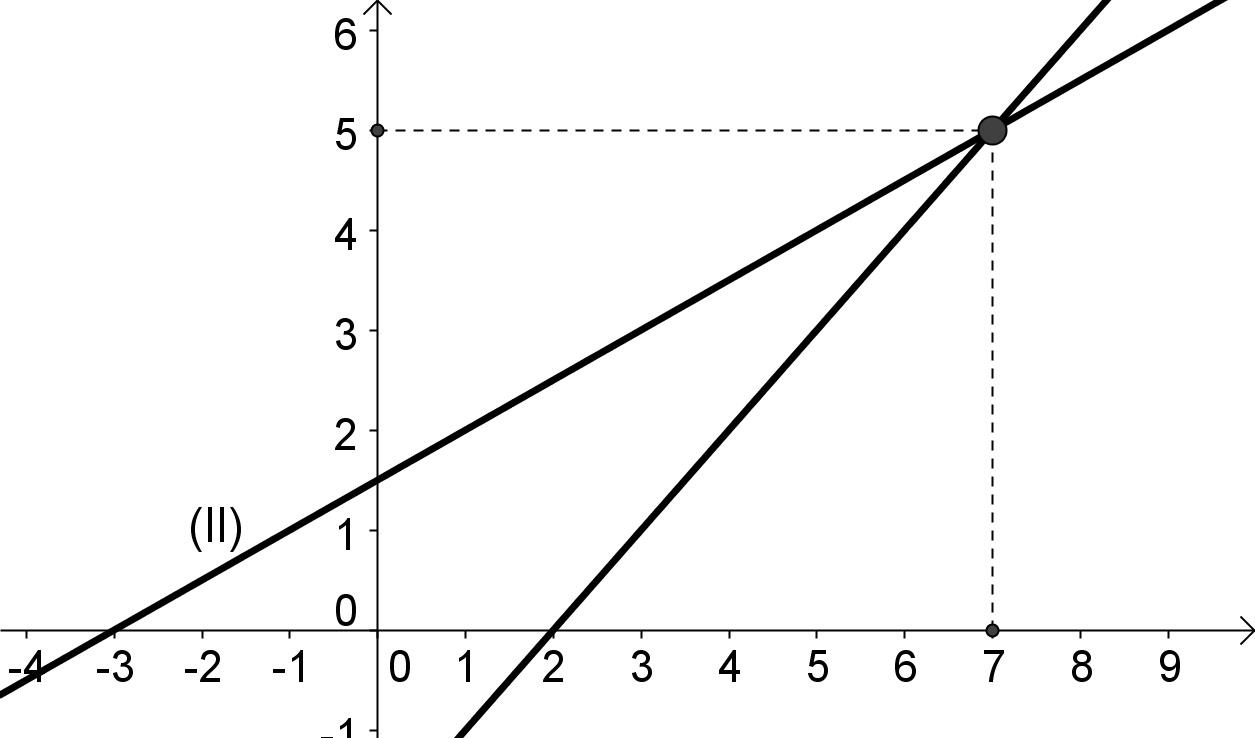
\includegraphics[height=7cm]{ZweiGeraden}}
\end{center} 
\end{figure}

\begin{remark}
You probably remember from the Bezirkschule that for $y=ax+b$, $a$ denotes the gradient of the line and $b$ denotes the $y$-axes-interception.
\end{remark}

The two lines denote the set of all 2-tuples $(x/y)$ which fulfil the two equations (I) and (II). The intersection point of the two lines stands for the only point which fulfils both equations and is therefore the solution of the system of linear equations. 
\vsp

We can see in the above sketch that $(7/5)$ is the intersection point of the two lines and therefore $x=7, y=5$ is the solution of the above system of linear equations.


\newpage
\begin{exer}
$ $

\begin{enumerate}[label=\emph{\alph*})]
\item	Solve the following system of linear equations geometrically:
\[
\begin{array}{lrcl}
(I)&-2x+5&=&y+2\\
(II)&4x-4y&=&12\\
\end{array}
\]		 

\begin{center}
\setlength{\unitlength}{0.75cm}
\begin{picture}(15,14)
\linethickness{0.03mm}

%\put(8,3){\circle*{0.2}}

\multiput(0,0)(1,0){16}%
{\line(0,1){13}}

\multiput(0,0)(0,1){14}%
{\line(1,0){15}}
\thicklines
%\linethickness{0.3mm}
%\put(7,0){\vector(0,1){13}}
%\put(0,2){\vector(1,0){16}}

\end{picture}
\end{center}
\vfill

\item	If the two lines are parallel, the lines do not intersect and there is no solution! Write down a system of linear equations with this property.
\vfill

\item	It could also be that there are infinitely many intersection points! How? Write down a system of linear equations with this property.
\vfill

\end{enumerate}
\end{exer}
\vfill

\begin{exer}
Think of a graphical solution for a $3\times 3$ SLE. What are the special cases in the 3-dimensional space?
\end{exer}
\vfill

\newpage
%%%%%%%%%%%%%%%%%%%%%%%%%%%%%%%%%%%%%%%%%%%%%%%%%%%%%
% Graphical Solution:1 ends here

% [[file:../index.org::*Singular SLE][Singular SLE:1]]
\subsection{Singular SLE}
% Singular SLE:1 ends here

% [[file:../index.org::*Linearly Dependent SLE][Linearly Dependent SLE:1]]
\subsubsection{Linearly Dependent SLE}

We learnt two methods how to solve a SLE. Nevertheless, things can go wrong sometimes:

\[
\begin{array}{lrcl}
(I)&3x&=&2y+3\\
(II)&x-\frac{2}{3}y&=&1\\
\end{array}
\]

At first glance everything is fine with this system of linear equations. But:

\[
(II) \hsp\Leftrightarrow\hsp 3x-2y=3 \hsp\Leftrightarrow\hsp 3x=2y+3 \hsp\Leftrightarrow\hsp (I)
\]

The two equations are actually equivalent, i.e. we may multiply one equation by a number to get exactly the other one. We get a $1\times 2$-system. This system has infinitely many solutions: $\left(0/-\frac{3}{2}\right)$, $(1/0)$ or $(3/3)$ are all solutions of the system and there are many more.
\vsp

From the graphical point of view this just means that we have twice the same line and therefore there are infinitely many intersection points.
\vsp

We can solve the one equation with respect to $x$ to get
\[
x=1+\frac{2}{3}y.
\]
We get the solution set
\[
\left\{(x/y) \in \R^2 \mid x=1+\frac{2}{3}y\right\} \hsp\hsp\text{ or } \hsp\hsp (1+\frac{2}{3}\lambda / \lambda) \text{ for all } \lambda \in \R.
\]

\begin{tcolorbox}[colback=white]\begin{definition}
If we are able to transform an equation by linear operations into another one, we call the two equations \textbf{linearly dependent}. If a system of linear equations contains linearly dependent equations we call the SLE \textbf{linearly dependent}, too.
\end{definition}
\end{tcolorbox}
\vsp

\begin{example}

\[
\begin{array}{lrcl}
(I)&x+y+z&=&5\\
(II)&x+2y-3z&=&10\\
(III)&2x+3y-2z&=&15\\
\end{array}
\]
Add (I) and (II) we get the equation (III). The SLE is linearly dependent and we can omit the third equation, since the information of the third equation is already contained in the first two equations. The SLE is therefore equivalent to
\[
\begin{array}{lrcl}
(I)&x+y+z&=&5\\
(II)&x+2y-3z&=&10\\
\end{array}
\]
Solving the first equation $(I)$ with respect to $x$ we get $x=5-y-z$ $(I')$. Inserting this solution into $(II)$ gives
\[
5-y-z+2y-3z=10 \hsp\Leftrightarrow\hsp y-4z=5 \hsp\Leftrightarrow\hsp y=5+4z
\]
Replacing $y$ in $(I)'$ results in
\[
x=5-(5+4z)-z=-5z.
\]
The solution is therefore 
\[
\left(-5\lambda / 5+4\lambda / \lambda \right) \hsp\text{ for } \lambda \in \R
\]
or similarly
\[
\mathbb{L}=\left\{(x/y/z)\in \R^3\mid x=-5z \text{ and } y=5+4z)\right\}.
\]

\end{example}
\vsp


%%%%%%%%%%%%%%%%%%%%%%%%%%%%%%%%%%%%%%%%%%%%%%%%%%%%%%%%%%%%%%%%%%R
% Linearly Dependent SLE:1 ends here

% [[file:../index.org::*Inconsistent SLE][Inconsistent SLE:1]]
\subsubsection{Inconsistent SLE}
We consider the following SLE:
\[
\begin{array}{lrcl}
(I)&2x-y&=&5\\
(II)&2y&=&7+4x\\
\end{array}
\]
Notice that
\[
(II) \hsp\Leftrightarrow\hsp -7=4x-2y \hsp\Leftrightarrow\hsp 2x-y=-3.5
\]

and therefore we get the equivalent system
\[
\begin{array}{lrcl}
(I)&2x-y&=&5\\
(II)'&2x-y&=&-3.5\\
\end{array}
\]

The two equations contradict each other! There is no solution. Geometrically this means that the two lines are parallel and therefore there is no intersection point and 
\[
\mathbb{L}=\emptyset.
\]


\begin{tcolorbox}[colback=white]
\begin{definition}
Two equations of a SLE are called \textbf{inconsistent} if they contradict each other.
\end{definition}
\end{tcolorbox}
\vsp\vsp

\begin{tcolorbox}[colback=white]
\begin{theorem}
A SLE has either one, no or infinitely many solutions. A SLE which has either no or infinitely many solutions is called \textbf{singular}. A SLE with exactly one solution is called \textbf{regular}.

\end{theorem}
\end{tcolorbox}


\newpage
% Inconsistent SLE:1 ends here

% [[file:../index.org::*Exercises][Exercises:1]]
\subsubsection{Exercises}
\begin{exer}
Solve the following linearly dependent SLE and write down its solution set:
\[
\begin{array}{lrcl}
(I)&x+y&=&1\\
(II)&2y&=&2-2x\\
\end{array}
\]
\end{exer}
\vfill

\begin{exer}

Which of the following systems are singular? Solve all of them and write down the solution set. Notice that some of them don't seem to be linear systems. But you can always transform them in a way such that you get a system of linear equations. 

\begin{enumerate}[label=\emph{\alph*})]
\item
\begin{itemize}
\item[(I)] $x+3y=4$
\item[(II)] $2x-y=1$
\end{itemize}
\vfill

\item
\begin{itemize}
\item[(I)] $\frac{x+3}{4}=\frac{2y-1}{6}$
\item[(II)] $3x-4y=2$
\end{itemize}
\vfill

\newpage
\item
\begin{itemize}
\item[(I)] $\frac{x+2}{4}-\frac{y-2}{12}=1.25$
\item[(II)] $y=3x-7$
\end{itemize}
\vfill

\item
\begin{itemize}
\item[(I)] $(x+3)(y+6)=(x+6)(y+4)$
\item[(II)] $(x-9)(y-8)=(x-15)(y-4)$
\end{itemize}
\vfill


\item
\begin{itemize}
\item[(I)] $\frac{1}{y+1}+\frac{1}{y-1}=\frac{10-x}{y^2-1}$
\item[(II)] $\frac{1}{x-2}+\frac{3}{y-4}=\frac{5}{2-x}$
\end{itemize}
\vfill

\newpage
\item
\begin{itemize}
\item[(I)] $x=ay+b$
\item[(II)] $y=a+by$
\end{itemize}
\vfill


\item
\begin{itemize}
\item[(I)] $ax+by=2a$
\item[(II)] $a^2x+b^2y=a^2+b^2$
\end{itemize}
\vfill

\end{enumerate}
\end{exer}

\newpage
% Exercises:1 ends here

% [[file:../index.org::*Coefficient matrix][Coefficient matrix:1]]
%%%%%%%%%%%%%%%%%%%%%%%%%%%%%%%%%%%%%%%%%%%%%%%%%%%%% 
\subsection{\tr|The Coefficient Matrix|Die Koeffizientenmatrix|}

\tr|The methods we used so far involve a lot of writing. You might have realized how often you simply copy the variables.
    In addition it is not at all obvious how to write a program that solves a linear system.  
   |Die bisher erarbeiteten Methoden zur Lösung eines LGS bedeuten einen grossen Schreibaufwand.
    Zudem ist nicht offensichtlich, wie sie in ein Rezept (einen Algorithmus) umgewandelt werden können,
    welchem auch eine Maschine (z.B. ein Computer) problemlos folgen kann. |
\tr|
   |
    \begin{tcolorbox}[colback=white]\begin{definition} 
    Ein \textbf{Algorithmus} ist ein automatisierbares Verfahren, das in endlich vielen Schritten einen Input zu einem Output verarbeitet. 
    Dabei muss jeder Schritt aus einer eindeutigen Anweisung bestehen, die programmierbar ist. 
    \end{definition}
    \end{tcolorbox}
    Idealerweise mündet ein Algorithmus in ein Computerprogramm, welches das Problem ohne weiteres menschliches Zutun automatisch löst. 
    \vsp
    |
\subsubsection*{\tr|How can we eliminate both problems at once?
  |Wie können wir diese zwei Nachteile (grosser Schreibaufwand und nicht offensichtlicher Algorithmus) beheben?| }

\tr|
   |Die sogenannte Gauss-Elimination liefert ein Algorithmus, der zu einem LGS (als Input) das Lösungstupel berechnet oder aber aufzeigt, dass das System singulär ist.
   In der hier vorgestellten Form geht der Algorithmus zurück auf den berühmten deutschen Mathematiker C. F. Gauss (1777-1855). |
\vsp

\tr|First of all we will minimize notational overhead. 
   |Zunächst minimieren wir den Schreibaufwand, indem wir von einem LGS nur das Allernötigste notieren.|

\begin{example}
\[
\begin{array}{rcl}
2x+4y-3z&=&-7\\
x+y+6z&=&1\\
-x+2y+3z&=&-4\\
\end{array}
\]
\end{example}
	 
\tr|From now on we will write all equations in normal form. In addition we fix some order for the variables (e.g. lexikogrgaphical order)
    We also want to get rid of the '+' and '-' signs, hence we have to make sure that there are only '+' signs. If there happens to be a '-' sign we simply
    attach it to the constant factor in front of the following variable (and invent a factor 1 if necessary).
   |Wir schreiben ab jetzt Gleichungen immer zuerst in der \glqq Normalform \grqq,
   wobei wir zusätzlich die Variablen in lexikographischer Reihenfolge schreiben und nur Pluszeichen (keine Minuszeichen, respektive wir nehmen das Minus zur Zahl) verwenden:|
\[
\begin{array}{rcl}
2x+4y+(-3)z&=&-7\\
x+y+6z&=&1\\
(-1)x+2y+3z&=&-4\\
\end{array}
\]
\vsp

\trx;We represent the position of the =  sign with a vertical bar. 
    ;Nun genügt es, die Koeffizienten aufzuschreiben, um das System eindeutig zu repräsentieren:;
\[
\left[\begin{array}{rrr|r}
2&4&-3&-7\\
1&1&6&1\\
-1&2&3&-4
\end{array}\right]
\]

	 
\tr|We can reconstruct the original linear system from this representation, but we got rid of all variables, '=' and  '+' signs. 
   |Aus dieser Darstellung kann das LGS eindeutig rekonstruiert werden, aber wir sparen beim Aufschreiben alle Variablen, Gleichheits- und Operationszeichen ein.|

\begin{tcolorbox}[colback=white]
\begin{definition}
\tr|For a  $m\times n$ linear system in \textbf{normalform} 
   |Ein $m\times n$-LGS liegt in \textbf{Normalform} vor, genau dann wenn es folgende Form hat:|

\[
\begin{array}{rcl}
a_{1,1}x_1+a_{1,2}x_2+\ldots+a_{1,n}x_n&=&b_1\\
a_{2,1}x_1+a_{2,2}x_2+\ldots+a_{2,n}x_n&=&b_2\\
&\cdots&\\
a_{m,1}x_1+a_{m,2}x_2+\ldots+a_{m,n}x_n&=&b_m\\
\end{array}
\] 
\vsp

\trx;we define the \textbf{extended coefficient matrix} to be the following scheme:
    ;Unter der \textbf{erweiterten Koeffizientenmatrix} versteht man die schematische Darstellung aller Koeffizienten und Konstanten in der Form;
\[
\left[\begin{array}{llll|l}
a_{1,1}&a_{1,2}&\cdots&a_{1,n}&b_1\\
a_{2,1}&a_{2,2}&\cdots&a_{2,n}&b_2\\
&&\cdots&&\\
a_{m,1}&a_{m,2}&\cdots&a_{m,n}&b_m\\
\end{array}\right]
\]
\tr|The 'extended' refers to the fact that the matrix also contains the $b$ paramters. Without this last column the matrix is usually called the 'coefficient matrix'.
    We take the liberty to omit the 'extended' if it is clear form the context which matrix we mean.
   |Der Zusatz 'erweitert' bezieht sich auf die Tatsache, dass die Matrix auch die $b$ Paramaterin der letzen Spalte enthält. Ohne diese letzte Spalte nenn man die Matrix
    üblicherweise nur die 'Koeffizienten Matrix'. Wir werden den Zusatz 'erweitert' manchmal weglassen, wenn klar ist, welche Matrix gemeint ist.|
\end{definition} 

\end{tcolorbox}



%\begin{remark}
%\tr|We can reconstuct the original linear system form the coefficient matrix.
%   |Aus der erweiterten Koeffizientenmatrix ist das LGS eindeutig rekonstruierbar.|
%\end{remark}
%\vsp

\begin{exer}
\tr|Consider exercises \ref{Uebungen2} a)-e) on page \pageref{Uebungen2}. Write down the coefficient matrix for each of these lienear systems. 
   |Betrachten Sie die Übungen a)-e) auf Seite \pageref{Uebungen2}.  Notieren Sie zu jedem dort gezeigten LGS die erweiterte Koeffizientenmatrix!|
\end{exer}
\par\medskip
\tr|So far we have only reduced the notational overhead; but the system is not yet solved.
    Our goal is to transform the coefficient matrix into an equivalent one that is either easier to solve
    or where we can simply read off the solution.
   |Nun haben wir erst den Schreibaufwand reduziert; das System ist aber noch nicht gelöst.
    Das Ziel ist, die erweiterte Koeffizientenmatrix so zu verarbeiten, dass daraus ein zum ursprünglichen System \glqq äquivalentes \grqq$ $ System resultiert,
    das ganz leicht lösbar ist oder aus dem die Lösung sogar sofort ablesbar ist.|

\begin{tcolorbox}[colback=white]
\begin{definition}
  \tr|Two linear systems are called \textbf{equivalent} if they do have the same solutions.
     |Ein LGS heisst \textbf{äquivalent} zu einem anderen LGS, wenn beide dieselbe Lösungsmenge haben.|
\end{definition}
\end{tcolorbox}




\newpage
%%%%%%%%%%%%%%%%%%%%%%%%%%%%%%%%%%%%%%%%%%%%%%%%%%%%% 

\subsection{\tr|Gauss eliminatin for non-singular linear systems|Die Gauss-Elimination für Nicht-singuläre LGSe|}

\begin{exer}$ $
\begin{itemize}
\item[a)] \tr|Consider the following linear systems:|Betrachten Sie folgendes LGS:|
\[
\begin{array}{rcl}
4x_1-5x_2+x_3&=&-9\\
3x_2+4.5x_3&=&4\\
6x_3&=&-12\\
\end{array}
\] 
\tr|Write down the extended coefficient matrix und explain why this system is probably easy to solve because of its special form.
   |Notieren Sie die erweiterte Koeffizientenmatrix, und erklären Sie, weshalb dieses System im Hinblick auf die Erarbeitung der Lösung in einer besonders glücklichen Form ist.|

\vfill

\item[b)]\tr|Consider the following linear systems:|Betrachten Sie folgendes LGS:|
\[
\begin{array}{rcl}
4x_1&=&-9\\
3x_2&=&4\\
6x_3&=&-12\\
\end{array}
\] 
 

\tr|Write down the extended coefficient matrix und explain why this system is probably even easier to solve because of its special form.
   |Notieren Sie die erweiterte Koeffizientenmatrix, und erklären Sie, weshalb dieses System im Hinblick auf die Erarbeitung der Lösung in einer noch glücklicheren Form ist.|
\vfill


\item[c)]\tr|Consider the following linear systems:|Betrachten Sie folgendes LGS:|
\[
\begin{array}{rcl}
x_1&=&-9\\
x_2&=&4\\
x_3&=&-12\\
\end{array}
\] 
\tr|Write down the extended coefficient matrix und explain why this system is probably the easiest to solve because of its special form.
   |Notieren Sie die erweiterte Koeffizientenmatrix, und erklären Sie, weshalb dieses System im Hinblick auf die Erarbeitung der Lösung in der glücklichsten aller Formen ist.|
\end{itemize}
\end{exer}
\vfill

\newpage
 



\begin{center}
\framebox{\rule{0cm}{5mm}
\parbox{\textwidth}{

\begin{definition}
  \tr|A matrix with only zeros below the main diagonal (the diagonal from the upper left to the lower right corner) is said to be in \textbf{triangular form}. 
     |Eine Matrix, die links unterhalb der Hauptdiagonalen (die Diagonale von oben links nach unten rechts) ausschliesslich Nullen aufweist, befindet sich in der sogenannten \textbf{Treppenform}. |
\begin{eqnarray*}
\left[\begin{array}{rrrr|r}
*&\cdots&\cdots&\cdots&\cdots\\
0&*&\cdots&\cdots&\cdots\\
0&0&*&\cdots&\cdots\\
0&0&0&*&\cdots\\
\end{array}\right]
\end{eqnarray*}
\end{definition}
}}\end{center}

\begin{exer}
\tr|Write down an example of a $4\times 4$ coefficient matrix in triangular form.| Schreiben Sie ein Beispiel einer Koeffizientenmatrix eines $4\times 4$-LGS in Treppenform auf.|
\end{exer}
\vspace{4cm }
%\begin{example}
%\begin{eqnarray*}
%\left[\begin{array}{rrrr|r}
%2&-3&1&1&5\\
%0&5&-1&2&2\\
%0&0&1&-4&6\\
%0&0&0&4&1\\
%\end{array}\right]
%\end{eqnarray*}
%\end{example}

\begin{center}
\framebox{\rule{0cm}{5mm}
\parbox{\textwidth}{

\begin{definition}
\tr|A $m\times (m+1)$ matrix with ones on the main diagonal, some unspecified numbers in the last column and zeros everywhere else is said to be in \textbf{reduced triangular form}.
   |Eine $m\times (m+1)$-Matrix in Treppenform, die in der Hauptdiagonalen ausschliesslich Einsen, in der letzten Spalte irgendwelche Zahlen und sonst nur Nullen aufweist,
    befindet sich in der \textbf{reduzierten Treppenform}. |
\begin{eqnarray*}
\left[\begin{array}{rrrr|r}
1&0&0&0&\cdots\\
0&1&0&0&\cdots\\
0&0&1&0&\cdots\\
0&0&0&1&\cdots\\
\end{array}\right]
\end{eqnarray*}


\end{definition}
}}\end{center}

\begin{exer}
\tr|Write down an example of $4\times 4$ coefficient matrix in reduced triangular form. |Schreiben Sie ein Beispiel einer Koeffizientenmatrix eines $4\times 4$-LGS in reduzierter Treppenform auf.|
\end{exer}
\vspace{4cm}

\newpage

\begin{exer}
$ $

\begin{itemize}
\item[a)] \tr|Solve the following linear system:|Finden Sie die Lösung des folgenden LGS: |

$
\left[\begin{array}{rrrr|r}
1&0&0&0&-2\\
0&1&0&0&5\\
0&0&1&0&3\\
0&0&0&1&4\\
\end{array}\right]
$
\vsp\vsp\vsp

\item[b)]	\tr|Solve the following linear system:|Finden Sie die Lösung des folgenden LGS: |

$
\left[\begin{array}{rrrr|r}
2&-3&1&1&5\\
0&5&-1&2&2\\
0&0&1&-4&6\\
0&0&0&4&1\\
\end{array}\right]
$
\end{itemize}
\end{exer}
\vsp\vsp\vsp



\vsp

\underline{\tr|The main question is :|Nun stehen wir vor folgender zentralen Frage:|}

\tr|Can we transform the coefficient matrix of a given linear system algorithmically in such a way, that we end up with  reduced triangular matrix where we can read off the solution?
    In addition we should also be able to see whether the system is singular.
   |Wie können wir die erweiterte Koeffizientenmatrix irgend eines LGS so algorithmisch umformen, dass wir eine reduzierte Treppenform zum Herausfinden der Lösung vor uns haben?
   Zusätzlich sollten wir auch einfach erkennen können, ob und weshalb ein LGS singulär ist. |

\begin{exer}
\tr|Think about this question for a moment. How can we transform the equations of a linear system without changing its solutions. 
   |Denken Sie einen Moment über diese Frage nach! Überlegen Sie, welche Umformungen wir mit den Gleichungen eines LGS machen dürfen,
    ohne dabei die Lösungsmenge zu verändern -- sprich, um ein äquivalentes LGS zu erhalten. |
\end{exer}

\newpage

\tr||Wir bemerken folgendes:|
\begin{itemize}
\item \tr|The solutions of a linear system do not change if we exchange two equations (i.e. if we change the order of the equations).
         |Die Lösungsmenge eines LGS verändert sich nicht, wenn wir zwei Gleichungen vertauschen (d.h. die Gleichungen in einer anderen Reihenfolge schreiben). |
\begin{exer}
\tr|What is the impact of exchanging two equations on the coefficient matrix?
   |Welche Konsequenz hat die Vertauschung zweier Gleichungen in einem Gleichungssystem auf die erweiterte Koeffizientenmatrix? Machen Sie ein Beispiel mit einem $3\times 3$-LGS.|
\end{exer}
\vfill

\item \tr|The solutions of a linear system do not change if we multiply one of the equations with a number different from zero.
         |Die Lösungsmenge eines LGS verändert sich nicht, wenn wir eine Gleichung mit einer Zahl ungleich Null multiplizieren. |
\begin{exer}
\tr|What is the impact of multplying an equation with a number on the coefficient matrix?
   |Welche Konsequenz hat die Multiplikation einer Gleichung mit einer Zahl ungleich Null auf die erweiterte Koeffizientenmatrix? Machen Sie ein Beispiel mit einem $3\times 3$-LGS.|
\end{exer}
\vfill

\item \tr|The solutions of a linear system do not change if we add one equation to another (see 'elimination method').
         |Die Lösungsmenge eines LGS verändert sich nicht, wenn wir eine unserer Gleichungen zu einer anderen addieren (siehe Additionsmethode). |
\begin{exer}
\tr|What is the impact of adding one equation to another on the coefficient matrix?
   |Welche Konsequenz hat die Addition einer der Gleichungen zu einer anderen auf die erweiterte Koeffizientenmatrix? Machen Sie ein Beispiel mit einem $3\times 3$-LGS.|
\end{exer}
\end{itemize}
\vfill

\newpage
\tr|None of these operations actually changes the solutions, hence no combination of these operations does.
    Accordingly, we can change the coefficient matrix of a linear system without changing the solutions.
    The coefficient matrix is \textbf{invariant} under these operations.
   |Keine dieser drei Operationen ändert die Lösungsmenge. Also ändert auch eine beliebige Kombination dieser drei Operationen die Lösungsmenge nicht.
    Entsprechend dürfen wir die zu einem LGS gehörige Koeffizientenmatrix mit den obigen drei Operationen verändern, um die Lösung eines LGS zu finden.
    Wir sagen, die Koeffizientenmatrix sei bezüglich dieser drei Operationen \textbf{invariant}:|

%\begin{center}
%\framebox{\rule{0cm}{5mm}
%\parbox{\textwidth}{
%
%\begin{definition}
%Ändert sich die Lösungsmenge eines LGS unter einer wohldefinierten Operation nicht, so sagen wir, das LGS, respektive die Koeffizientenmatrix, sei unter dieser Operation \textbf{invariant}. 
%\end{definition}
%}}\end{center}


\vsp

\begin{tcolorbox}[colback=white]
\begin{theorem}
\tr|We can always reduce the coefficient matrix of a non-singular $n\times n$ system to reduced triangular form using only the following operations:
   |Die erweiterte Koeffizientenmatrix eines nicht-singulären $n\times n$-LGS kann immer anhand folgender Operationen in die reduzierte Treppenform überführt werden:|
\begin{itemize}
\item Operation 1: \tr|Exchanging two rows|Vertauschung zweier Zeilen|
\item Operation 2: \tr|Multiplying one row with an non-zero number|Multiplikation einer Zeile mit einer Zahl ungleich null|
\item Operation 3: \tr|Adding one row to another|Addition einer Zeile zu einer anderen Zeile|
\end{itemize}
\end{theorem}
\end{tcolorbox}



\begin{proof}
\tr|Somewhere in the first column has to be a non-zero entry, otherwise this wouldn't be a $n\times n$ system.
    Using operation 1 we can make sure that the element in the upper left corner is non-zero. 
   |Die erste Spalte besteht nicht nur aus Nullen, da es sich sonst nicht um ein $n\times n$-LGS handelt. Anhand von Operation 1 können wir dafür sorgen, dass oben links eine Zahl ungleich Null steht:|
\begin{eqnarray*}
\left[\begin{array}{rrrr|r}
a\neq 0& \cdots&\cdots&\cdots&\cdots\\
\cdots&\cdots&\cdots&\cdots&\cdots\\
\cdots&\cdots&\cdots&\cdots&\cdots\\
\cdots&\cdots&\cdots&\cdots&\cdots\\
\end{array}\right]
\end{eqnarray*}
\tr|Using operation 2 we can arrange 1 in the upper left corner.|Anhand von Operation 2 können wir oben links eine 1 erreichen:|
\begin{eqnarray*}
\left[\begin{array}{rrrr|r}
1& \cdots&\cdots&\cdots&\cdots\\
\cdots&\cdots&\cdots&\cdots&\cdots\\
\cdots&\cdots&\cdots&\cdots&\cdots\\
\cdots&\cdots&\cdots&\cdots&\cdots\\
\end{array}\right]
\end{eqnarray*}
\tr|Repeated application of operation 2 and 3 produces 0's under this 1.|Mehrmalige Anwendung von Operation 2 und 3 erzeugt unter der 1 Nullen.|
\begin{eqnarray*}
\left[\begin{array}{rrrr|r}
1& \cdots&\cdots&\cdots&\cdots\\
0&\cdots&\cdots&\cdots&\cdots\\
0&\cdots&\cdots&\cdots&\cdots\\
0&\cdots&\cdots&\cdots&\cdots\\
\end{array}\right]
\end{eqnarray*}
\tr|The first colums now has the desired shape and we won't change it in the next steps.
    From now on we ignore the first columns and the first row and consider the remaining $(n-1) \times n-1$ matrix.
   |Ab jetzt ändern und benutzen wir die erste Spalte nicht mehr. Sie ist bereits in der Form, welche wir uns wünschen.
    Wir betrachten nun die $(n-1)\times (n-1)$-Matrix, welche entsteht durch ignorieren der ersten Spalte und ersten Zeile:|

\setlength{\unitlength}{1cm}
\begin{picture}(1,1)
\put(5.5,-0.7){\line(5,0){4.5}}
\put(6.1,-2.7){\line(0,5){2.5}}
\end{picture}
\begin{eqnarray*}
\left[\begin{array}{rrrr|r}
1& \cdots&\cdots&\cdots&\cdots\\
0&\cdots&\cdots&\cdots&\cdots\\
0&\cdots&\cdots&\cdots&\cdots\\
0&\cdots&\cdots&\cdots&\cdots\\
\end{array}\right]
\end{eqnarray*}

\tr|In this smaller matrix we have to find again a non-zero element in the first column.
    This has to be possible because otherwise the second variable would have appeared only in the first equation of the original linear system.
    But in this case we could simply solve the smaller system, choose the second variable arbitrary and use the original first row to determine the first variable.
    But with a free variable the system would be singular contrary to our assumptions.
   |In dieser Restmatrix müssen wir nun erneut in der ersten Spalte (also in der zweiten Spalte der ursprünglichen Matrix) einen Eintrag ungleich null finden.
   Dies ist möglich, weil sonst die zweite Variable nur in der ersten Gleichung des LGS vorgekommen wäre und somit entweder die erste oder die zweite Variable frei gewählt werden könnte.
   Dann wäre das System aber singulär, aber wir gehen von einem nicht-singulären LGS aus.
   Durch Anwendung von Operation 1 können wir also in der Restmatrix folgende Form erhalten: |
\begin{eqnarray*}
\left[\begin{array}{rrr|r}
b\neq 0&\cdots&\cdots&\cdots\\
\cdots&\cdots&\cdots&\cdots\\
\cdots&\cdots&\cdots&\cdots\\
\end{array}\right]
\end{eqnarray*}
\tr|As before we can use operations 2 and 3 to produce zeros below $b$ and using operation 2 we can turn $b$ into a 1.
    Note that these operations do not alter the first row or the first column (why?). Our original matrix now looks like:
   |Nun können wir wieder durch gleiche Argumentation wie oben durch Anwendung von Operation 2 und 3 unterhalb von $b$ alles Nullen erreichen und durch Anwendung von Operation 2 aus $b$ eine 1 machen.
   Beachten Sie, dass diese Operationen die erste Zeile und erste Spalte unserer Orginalmatrix nicht verändern (Wieso?)! Unsere Orginalmatrix sieht nun wie folgt aus: |
\begin{eqnarray*}
\left[\begin{array}{rrrr|r}
1& \cdots&\cdots&\cdots&\cdots\\
0&1&\cdots&\cdots&\cdots\\
0&0&\cdots&\cdots&\cdots\\
0&0&\cdots&\cdots&\cdots\\
\end{array}\right]
\end{eqnarray*}

\tr|Again, we can use operations 1-3 to turn all entries on the diagonal into 1's and all entries below the diagonal into 0's.
   |Entsprechend können wir durch Anwendung von Operation 1-3 alle Diagonalelemente zu 1 und alle Einträge unterhalb den Einsen zu Null machen:|
\begin{eqnarray*}
\left[\begin{array}{rrrr|r}
1& \cdots&\cdots&\cdots&\cdots\\
0&1&\cdots&\cdots&\cdots\\
0&0&1&\cdots&\cdots\\
0&0&0&1&\cdots\\
\end{array}\right]
\end{eqnarray*}
\tr|We have reached triangular form. Again, using operations 2 and 3 we can produce a 0 in the second to last row above the 1. 
   |Die Treppenform ist erreicht. Durch Anwenden von Operation 2 und 3 können wir nun in der zweitletzten Zeile oberhalb der 1 alles Nullen erzeugen. |
\begin{eqnarray*}
\left[\begin{array}{rrrr|r}
1& \cdots&\cdots&0&\cdots\\
0&1&\cdots&0&\cdots\\
0&0&1&0&\cdots\\
0&0&0&1&\cdots\\
\end{array}\right]
\end{eqnarray*}
\tr|And of course we can do the same with all other rows. Finally we have reached reduced triangular form.
   |Und entsprechend auch bei allen anderen 1 oberhalb Nullen erzeugen, so dass wir die reduzierte Treppenform erreichen:|
\begin{eqnarray*}
\left[\begin{array}{rrrr|r}
1&0&0&0&\cdots\\
0&1&0&0&\cdots\\
0&0&1&0&\cdots\\
0&0&0&1&\cdots\\
\end{array}\right]
\end{eqnarray*}
\qed
\end{proof}

\vsp\vsp

\tr|This proof does not just prove our claim, in addition it also provides a medthod to transform a non-singular coefficient matrix into reduced triangular form.
    This method is called \textbf{Gauss-elimination}.
   |Dieser Beweis gibt uns nicht nur den Beweis für den Satz: Er zeigt uns auch gleich noch, wie wir vorgehen müssen, um eine nicht-singulären Koeffizientenmatrix auf eine reduzierte Treppenform zu bringen.
    Wir nennen diesen Vorgang die \textbf{Gauss-Elimination}.|


\begin{exer}\label{exerTreppenform}$ $
\begin{itemize}
\item[a)]
  \tr|Solve the folowing system using Gauss-elimination: |Lösen Sie folgendes LGS mit Gauss-Elimination.|
\[
\begin{array}{rcl}
4x-3y&=&7\\
-3x+5y&=&3
\end{array}
\]
	 
\tr|The solution in $(4,3)$.|Als Lösung müssten Sie $(4/3)$ erhalten.|
\vfill

\item[b)]\tr|Solve the folowing system using Gauss-elimination: |Lösen Sie folgendes LGS mit Gauss-Elimination. Bringen Sie dazu das LGS in die reduzierte Treppenform:|
\[
\begin{array}{rcl}
5x+2y+3z&=&6\\
-x-4y+9z&=&12\\
-2x-5y-3z&=&0
\end{array}
\]
	
\tr|The solution in $(1,-1,1)$. |Als Lösung müssten Sie $(1/-1/1)$ erhalten.|
\vfill

\end{itemize}
\end{exer}

\newpage
\subsection{\tr|Gauss elimination for singular systems|Gauss-Elimination für singuläre LGS|}

\tr|So far we assumed applied Gauss-elimination on non-singular systems, but what happens if we apply this method to a singular system?|Was passiert, wenn wir die Gauss-Elimination auf ein singuläres System anwenden? |


\begin{exer}$ $
\begin{itemize}
\item[a)] \tr|The following system is singular. Apply Gauss-elimination to it and see what happpens: |Folgendes System ist singulär. Bearbeiten Sie es mit Gauss-Elimination. Was stellen Sie fest?:|
\[
\begin{array}{rcl}
5x-3y&=&4\\
-10x+6y&=&5
\end{array}
\]
\vspace{3cm}

\item[b)] \tr|The following system is singular. Apply Gauss-elimination to it and see what happpens: |Folgendes System ist singulär. Bearbeiten Sie es mit Gauss-Elimination. Was stellen Sie fest?:|
\[
\begin{array}{rcl}
7x-y+2z&=&4\\
-3x+2y-z&=&1\\
-14x+2y-4z&=&-8
\end{array}
\]
\vspace{3cm}

\item[c)] \tr|How can you use the triangular shape of a coefficient matrix to decide whether a system is singular? |Wie kann man aus der Treppenform ablesen, dass ein System singulär ist?|
\vspace{4cm}

\item[d)] \tr|How does the algorithm show whether there are infinitely many solution or none at all?|Wie zeigt uns der Algorithmus, ob es unendlich viele Lösungen oder gar keine Lösungen gibt?|
\vspace{4cm}

\end{itemize}
\end{exer}


\newpage
%%%%%%%%%%%%%%%%%%%%%%%%%%%%%%%%%%%%%%%%%%%%%%%%%%%%% 

\subsection{\tr|Exercises|Übungen|}
\begin{exer} \label{Uebungen2}

\tr|Solve the following linear systems using Gauss-elimination:|Lösen Sie die folgenden LGSe mit Gauss-Elimination:|
\begin{itemize}
\item[a)] 
\begin{itemize}
\item[(I)] $2x-y+2z=12$
\item[(II)] $6x-3y+z=11$
\item[(III)] $3x+y-3z=-11$
\end{itemize}
%\textbf{Lösung:} $\mathbb{L}=\{-5,\frac{2}{5},\frac{6}{5}\}$
\vsp

\item[b)] \begin{itemize}
\item[(I)] $x+y+z=4$
\item[(II)] $x+y=5$
\item[(III)] $y+z=1$
\end{itemize}
%\textbf{Lösung:} $\mathbb{L}=\{3,2,-1\}$
\vsp

\item[c)]
\begin{itemize}
 \item[(I)] $x-y+4z=1$
\item[(II)] $2z=3$
\item[(III)] $3x-3y+5z=0$
\end{itemize}
%\textbf{Lösung:} $\mathbb{L}=\{\}$
\vsp

\item[d)]
\begin{itemize}
\item[(I)] $3y-z=3$
\item[(II)] $2x-2y+z=-2$
\item[(III)] $4x+2y=1$
\end{itemize}
%\textbf{Lösung:} $\mathbb{L}=\{\}$
\vsp

\item[e)]
\begin{itemize}
\item[(I)] $x_1+x_2=0$
\item[(II)] $x_1+x_2+x_3=0$
\item[(III)]  $x_2+x_3+x_4=0$
\item[(IV)] $x_3+x_4+x_5=0$
\item[(V)] $x_4+x_5=0$
\end{itemize}

%\textbf{Lösung:}
%\[
%\left[\begin{array}{ccccc|c}
%1 & 1 & 0 & 0 & 0 & 0\\
%1 & 1 & 1 & 0 & 0 & 0\\
%0 & 1 & 1 & 1 & 0 & 0\\
%0 & 0 & 1 & 1 & 1 & 0\\
%0 & 0 & 0 & 1 & 1 & 0
%\end{array}\right]
%\sim
%\left[\begin{array}{ccccc|c}
%1 & 1 & 0 & 0 & 0 & 0\\
%0 & 0 & 1 & 0 & 0 & 0\\
%0 & 1 & 1 & 1 & 0 & 0\\
%0 & 0 & 1 & 1 & 1 & 0\\
%0 & 0 & 0 & 1 & 1 & 0
%\end{array}\right]
%\sim
%\left[\begin{array}{ccccc|c}
%1 & 1 & 0 & 0 & 0 & 0\\
%0 & 1 & 1 & 1 & 0 & 0\\
%0 & 0 & 1 & 0 & 0 & 0\\
%0 & 0 & 0 & 1 & 1 & 0\\
%0 & 0 & 0 & 1 & 1 & 0
%\end{array}\right]
%\sim
%\left[\begin{array}{ccccc|c}
%51 & 1 & 0 & 0 & 0 & 0\\
%0 & 1 & 1 & 1 & 0 & 0\\
%0 & 0 & 1 & 0 & 0 & 0\\
%0 & 0 & 0 & 1 & 1 & 0\\
%0 & 0 & 0 & 0 & 0 & 0
%\end{array}\right]
%\]
%Es gibt also unendlich viele Lösungen.
\vsp

\item[f)]  \tr|The sum of two numbers is 17 and their difference is 7. Find these two numbers. |Die Summe zweier Zahlen ist 17 und ihre Differenz 7. Bestimme die Zahlen.|

%\textbf{Lösung:} Das zugehörige Gleichungssystem ist:
%\begin{itemize}
%\item[(I)]  $x+y=17$
%\item[(II)] $x-y=7$
%\end{itemize}
%Die Lösung ist $x=12$, $y=5$. Die Zahlen $12$ und $5$ erfüllen also die Bedingungen.
\vsp

\item[g)]
  \tr|A museum has different ticket fees for adults and children.  A couple and their four children pay 36 CHF. A woman whith three children pays 23 CHf. What are the fees for adults and children?
     |Das Verkehrshaus in Luzern hat unterschiedliche Eintrittspreise für Erwachsene und Kinder. Herr und Frau Schmidiger zahlen mit ihren vier Kindern 36 Franken Eintritt.
      Frau Vetter und ihre drei Kinder zahlen 23 Franken. Was kostet der Eintritt für Erwachsene und Kinder?|

%\textbf{Lösung:} $x$: Eintrittspreis für Erwachsene, $y$: Eintrittspreis für Kinder.
%\begin{itemize}
%\item[(I)]$2x+4y=36$
%\item[(II)] $x+3y=23$
%\end{itemize}
%Die Lösung ist $x=8$ und $y=5$. Erwachsene zahlen also $8$ Franken und Kinder $5$ Franken Eintritt.
\end{itemize}
\end{exer}




\newpage
%%%%%%%%%%%%%%%%%%%%%%%%%%%%%%%%%%%%%%%%%%%%%%%%%%%%%
% Coefficient matrix:1 ends here

% [[file:../index.org::*Non-quadratic systems: more or less equations than variables][Non-quadratic systems: more or less equations than variables:1]]
\subsection{\tr|Non-quadratic systems|Nicht quadratische Systeme|}
\tr|So far we only considered systems where we had equally many equations than variables. But in real life this is often not the case.
   |Bis jetzt haben wir uns nur quadratische Systeme angeschaut, mit gleichvielen Variabeln wie Gleichungen, aber in der Realität ist die oft nicht der Fall.|  
\begin{exer}
 \tr|Assume we have less equations than variables. What would the result of a Gauss-elimination look like?
    |Nehmen wir an, wir hätten weniger Gleichungen als Variabeln. Wie würde das Resultat einer Gauss-Elimination aussehen?|
\end{exer}
\vfill
\begin{exer}
 \tr|Assume we have more equations than variables. What would the result of a Gauss-elimination look like? Could you think of a situation where we still have exactly one solution?
    |Nehmen wir an, wir hätten mehr Gleichungen als Variabeln. Wie würde das Resultat einer Gauss-Elimination aussehen? Können Sie sich eine Situation vorstellen wo wir immer noch genau eine Lösung haben?|
\end{exer}
\vfill
% Non-quadratic systems: more or less equations than variables:1 ends here
